\subsection{Programmer und Debug Adapter (J-Link)}
\label{sec:SeggerJlink}

Um das DSP-Board zu flashen und debuggen kommt ein ARM Cortex fähiger Programmer zum Einsatz.
Dies kann beispielsweise ein ST-Link V2 von STMicroelectronics \cite{STLinkV2}, eine Black Magic Probe \cite{1bitBMP}.
In diesem Projekt kam ein \textit{J-Link EDU mini} von Segger\cite{JLinkEDU} zum Einsatz.
Der Einsatz dieses Programmers ist jedoch strikt auf den Gebrauch für Bildungszwecke eingeschränkt.

\subsubsection{J-Link Konfiguration in Keil uVision}

Damit der Flash-download und das Debugging richtig funktioniert, müssen in Keil uVision folgende Einstellungen vorgenommen werden.

\begin{figure}[H]
	\centering
	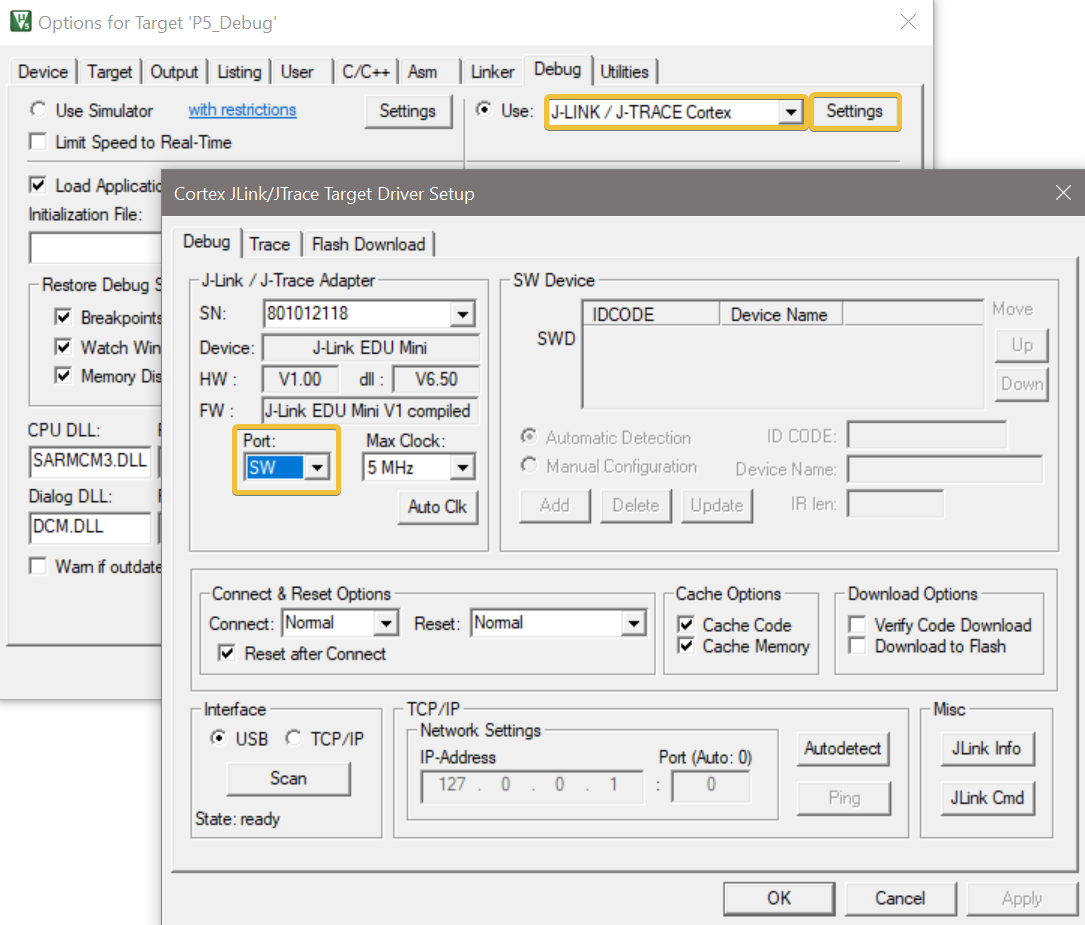
\includegraphics[width=0.9\linewidth]{keil-jlink}
	\caption{Project Properties mit den Einstellungen für den Segger J-Link im SWD Modus}
	\label{pic:keil-jlink}
\end{figure}

Die Abbildung \ref{pic:keil-jlink} zeigt das Fenster mit den Project Properties, das unter \texttt{Project > Options for Target 'DSP Board' > Debug} zu finden ist.
Hier muss "\textit{use J-Link/J-Trace}" ausgewählt und die Settings dazu geöffnet werden. 
Die Hardwareschnittstelle ist SWD und nicht JTAG.

